\documentclass{exam}

\usepackage{titling}
\usepackage{amsmath}
\usepackage{amsfonts}
\usepackage{mathtools}
\usepackage{float}
\usepackage{tikz}
\usepackage{graphicx}
\usepackage{subfig}
\usepackage{minted}
\usepackage{inconsolata}
\usepackage{tikz}
\usepackage[font={small}]{caption}

\graphicspath{ {./src/output} }


\setlength{\droptitle}{-5em}   


\renewcommand{\questionlabel}{\textbf{~\thequestion)}}
\renewcommand{\thepartno}{\roman{partno}}
\DeclarePairedDelimiterX{\norm}[1]{\lVert}{\rVert}{#1}

\newcommand*{\horzbar}{\rule[.5ex]{2.5ex}{0.5pt}}

\newenvironment{shiftedflalign*}{%
    \start@align\tw@\st@rredtrue\m@ne
    \hskip\parindent
}{%
    \endalign
}



\title{Homework 3 - Group 076}
\author{Aprendizagem 2021/2022}
\date{}

\cfoot{\thepage}

\begin{document}
    \maketitle
    \begin{tikzpicture}[overlay, remember picture]
        \node[xshift=3.5cm,yshift=-2cm] at (current page.north west) {
\includegraphics[scale = 0.35]{logo_ist.jpeg}};
    \end{tikzpicture}
    \vspace{-4.5em}
    \section{Pen and Paper}
    \begin{questions}
        \item Let $b^{[l]}$, $net^{[l]}$ and $a^{[l]} = \phi(net^{[l]})$ denote the vector of biases, net values and activations of the $l$-th layer, respectively (with $\phi_i(net^{[l]}) = \tanh(net_i^{[l]})$ being the activation function). Let $W^{[l]} = [w_{ij}]$ be the matrix of weights $w_{ij}$ that connect the $j$-th activation of layer $l-1$ to the $i$-th net of layer $l$.
        \begin{itemize}
            \item \textbf{Forward Propagation}
            \vspace{0.4em} \\
            Given that $a^{[l]} = \phi(net^{[l]}) = \phi(W^{[l]}a^{[l-1]} + b^{[l]})$ ($i \in \{1, 2, 3\}$), considering that $a^{[0]} = \mathbf{x}$:
            \begin{align*}
                a^{[1]} &= \phi(W^{[1]}a^{[0]} + b^{[1]}) = \phi\left(
                \begin{bmatrix}
                    1.0 & 1.0 & 1.0 & 1.0 & 1.0  \\
                    0.0 & 0.0 & 0.0 & 0.0 & 0.0  \\
                    1.0 & 1.0 & 1.0 & 1.0 & 1.0 
                \end{bmatrix} 
                \begin{bmatrix}
                    1  \\
                    1  \\
                    1  \\
                    1  \\
                    1  \\
                \end{bmatrix} + 
                \begin{bmatrix}
                    1.0  \\
                    1.0  \\
                    1.0  \\
                \end{bmatrix} \right) \\
                &= \phi\left(
                \begin{bmatrix}
                    6.0  \\
                    1.0  \\
                    6.0  \\
                \end{bmatrix}\right) = 
                \begin{bmatrix}
                    \tanh(6.0) \\
                    \tanh(1.0) \\
                    \tanh(6.0) \\
                \end{bmatrix} = 
                \begin{bmatrix}
                    0.99999  \\
                    0.76159  \\
                    0.99999  \\
                \end{bmatrix} \\
                a^{[2]} &= \phi(W^{[2]}a^{[1]} + b^{[2]}) = \phi\left(
                \begin{bmatrix}
                    1.0 & 1.0 & 1.0  \\
                    1.0 & 1.0 & 1.0  \\
                \end{bmatrix} 
                \begin{bmatrix}
                    0.99999  \\
                    0.76159  \\
                    0.99999  \\
                \end{bmatrix} + 
                \begin{bmatrix}
                    1.0  \\
                    1.0  \\
                \end{bmatrix} \right)
                = \phi \left(
                \begin{bmatrix}
                    3.76157  \\
                    3.76157  \\
                \end{bmatrix} \right) = 
                \begin{bmatrix}
                    0.99892  \\
                    0.99892  \\    
                \end{bmatrix} \\
                a^{[3]} &= \phi(W^{[3]}a^{[2]} + b^{[3]}) = \phi\left(
                \begin{bmatrix}
                    0.0 & 0.0  \\
                    0.0 & 0.0  \\
                \end{bmatrix} 
                \begin{bmatrix}
                    0.99892  \\
                    0.99892  \\
                \end{bmatrix} + 
                \begin{bmatrix}
                    0.0  \\
                    0.0  \\
                \end{bmatrix} \right) 
                = \phi \left(
                \begin{bmatrix}
                    0.0  \\
                    0.0  \\
                \end{bmatrix} \right) =
                \begin{bmatrix}
                    0.0  \\
                    0.0  \\   
                \end{bmatrix}
            \end{align*}

            \item \textbf{Backward propagation} \\
            Consider the squared error loss $E = \frac{1}{2}\sum_{i = 1}^{2} (\mathbf{z}_i - \mathbf{\hat{z}}_i)^2 = \frac{1}{2}\sum_{i = 1}^{2} \left(\mathbf{z}_i - a_i^{[3]}\right)^2 =  \frac{1}{2}\| \mathbf{z} - a^{[3]}\|^2$ and define $\delta^{[l]} = \nabla_{net^{[l]}} E$. By the chain rule of derivation, we have, for layer $l \in \{1, 2\}$, with $n_l$ denoting the number of units in layer $l$:
            \begin{align}
                \delta^{[l]}& = \nabla_{net^{[l]}} E = \nabla_{net^{[l]}} a^{[l]} \nabla_{a^{[l]}} net^{[l+1]} \nabla_{net^{[l+1]}} E  \nonumber \\
                &= \text{diag}(\tanh'(net^{[l]}_1), ..., \tanh'(net^{[l]}_{n_l}))(W^{[l + 1]})^T\delta^{[l + 1]} \nonumber \\
                &= 
                \begin{bmatrix}
                    \tanh'(net^{[l]}_1) & \cdots & \tanh'(net^{[l]}_{n_l})
                \end{bmatrix}^T \circ \left((W^{[l + 1]})^T\delta^{[l + 1]}\right) \nonumber \\
                &= \begin{bmatrix}
                    1 - \tanh^2(net^{[l]}_1) & \cdots &  1 - \tanh^2(net^{[l])}_{n_l}
                \end{bmatrix}^T \circ \left((W^{[l + 1]})^T\delta^{[l + 1]}\right) \nonumber \\
                &= \begin{bmatrix}
                    1 - (a^{[l]}_1)^2 & \cdots &  1 - (a^{[l]}_{n_l})^2
                \end{bmatrix}^T \circ \left((W^{[l + 1]})^T\delta^{[l + 1]}\right) \label{eq:1}
            \end{align}
            where in the two last steps the equalities $\tanh'(x) = 1 - \tanh^2(x)$ and $a^{[l]}_i = \tanh(net^{[l]}_i)$ were used. For the output layer ($l = 3$), using the equality $\nabla_x \left(\frac{1}{2}\|x\|^2\right) = x$ to compute $\nabla_{a^{[3]}}{E}$, we have:
            \begin{equation}
                \delta^{[3]} = \nabla_{net^{[3]}}{a^{[3]}} \nabla_{a^{[3]}}{E} = 
                \begin{bmatrix}
                    1 - (a^{[3]}_1)^2 &   1 - (a^{[3]}_{2})^2
                \end{bmatrix}^T \circ (\mathbf{z} - a^{[3]})
                \label{eq:2}
            \end{equation}
            Computing the deltas:
            \begin{align*}
                \delta^{[3]} = 
                \begin{bmatrix}
                    1.0  \\
                    1.0 \\
                \end{bmatrix} \circ
                \begin{bmatrix}
                    -1.0  \\
                    1.0  \\
                \end{bmatrix} = 
                \begin{bmatrix}
                    -1.0  \\
                    1.0  \\
                \end{bmatrix} \quad
                \delta^{[2]} &= 
                \begin{bmatrix}
                    0.0  \\
                    0.0  \\
                \end{bmatrix} \quad
                \delta^{[1]} = 
                \begin{bmatrix}
                    0.0  \\
                    0.0  \\
                    0.0
                \end{bmatrix}
            \end{align*} 
            since $W^{[3]}$ is a null matrix and $\delta^{[2]}$ is a null vector (so $\delta_{[2]}$ and $\delta_{[2]}$ are null according to \eqref{eq:1}).
            \item \textbf{Parameter update} \\
            To perform gradient descent on the weights and biases, we calculate the gradient of the error with respect to these parameters ($l \in \{1, 2, 3\}$):
            \begin{equation}
                \frac{\partial E}{\partial w_{ij}^{[l]}} = \frac{\partial E}{\partial net_{i}^{[l]}} \frac{\partial net_i^{[l]}}{\partial w_{ij}^{[l]}} = \delta_i^{[l]} a_j^{[l - 1]} \Rightarrow \nabla_{W^{[l]}} E = \delta^{[l]} (a^{[l - 1]})^{T} \label{eq:3}
            \end{equation}
            \begin{equation}
                \nabla_{b^{[l]}} E = \nabla_{b^{[l]}} net^{[l] }  \nabla_{net^{[l]}} E = \mathbb{I}^{n_l \times n_l} \delta^{[l]} = \delta^{[l]} \label{eq:4}
            \end{equation}
            since for $x, y \in \mathbb{R}^n$, we have that $xy^T = [x_i y_j]$. Thus, setting the learning rate  $\eta$ to 0.1:
            \begin{align*}
                \nabla_{W^{[3]}} E &= 
                \begin{bmatrix}
                    -1.0  \\
                    1.0  \\
                \end{bmatrix}
                \begin{bmatrix}
                    0.99892  & 
                    0.99892  
                \end{bmatrix} = 
                \begin{bmatrix}
                    -0.99892 & -0.99892  \\
                    0.99892 & 0.99892  \\
                \end{bmatrix} \\
                \nabla_{b^{[3]}} E &= 
                \begin{bmatrix}
                    -1.0  \\
                    1.0  \\
                \end{bmatrix} \\
                (W^{[3]})^{\text{new}} &= (W^{[3]})^{\text{old}} - \eta \nabla_{W^{[3]}} E = 
                \begin{bmatrix}
                    0.09989 & 0.09989  \\
                    -0.09989 & -0.09989  \\
                \end{bmatrix} \\
                (b^{[3]})^{\text{new}} &= (b^{[3]})^{\text{old}} - \eta \nabla_{b^{[3]}} E = 
                \begin{bmatrix}
                    0.1  \\
                    -0.1  \\
                \end{bmatrix}
            \end{align*}
            As deltas in layers 1 and 2 are zero valued vectors, the error gradient with respect to the weights and biases of these layers is also zero valued, acordding to \eqref{eq:3} and \eqref{eq:4}. Thus, these parameters don't change:
            \begin{equation*}
                \begin{split}
                    (W^{[2]})^{\text{new}} &= (W^{[2]})^{\text{old}} = 
                    \begin{bmatrix}
                        1.0 & 1.0 & 1.0  \\
                        1.0 & 1.0 & 1.0  \\
                    \end{bmatrix}  \\
                    (W^{[1]})^{\text{new}} &= (W^{[1]})^{\text{old}} = 
                    \begin{bmatrix}
                        1.0 & 1.0 & 1.0 & 1.0 & 1.0  \\
                        0.0 & 0.0 & 0.0 & 0.0 & 0.0  \\
                        1.0 & 1.0 & 1.0 & 1.0 & 1.0  \\
                    \end{bmatrix}
                \end{split} \quad
                \begin{split}
                    (b^{[2]})^{\text{new}} &= (b^{[2]})^{\text{old}} = 
                    \begin{bmatrix}
                        1.0  \\
                        1.0  \\
                    \end{bmatrix} \\
                    (b^{[1]})^{\text{new}} &= (b^{[1]})^{\text{old}} = 
                    \begin{bmatrix}
                        1.0  \\
                        1.0  \\
                        1.0  \\
                    \end{bmatrix}
                \end{split}
            \end{equation*}
        \end{itemize}
        \item { \; } 
            \begin{itemize}
                \item \textbf{Forward Propagation} \\
                The only change in this stage occurs in the activation function in the last layer, which is now softmax:
                \begin{equation*}
                    a^{[3]} = \text{softmax}(net^{[3]}) = \sigma(net^{[3]}) = \left(\frac{e^{net^{[3]}_1}}{\sum_{j = 1}^{2}e^{net^{[3]}_j}},\frac{e^{net^{[3]}_2}}{\sum_{j = 1}^{2}e^{net^{[3]}_j}}\right)
                \end{equation*}  
                And so we have:
                \begin{align*}
                    a^{[1]} = 
                    \begin{bmatrix}
                        0.99999  \\
                        0.76159  \\
                        0.99999  \\
                    \end{bmatrix} \quad 
                    a^{[2]} = 
                    \begin{bmatrix}
                        0.99892  \\
                        0.99892  \\   
                    \end{bmatrix} \quad 
                    a^{[3]} = \sigma(net^{[3]}) = \sigma\left(
                    \begin{bmatrix}
                        0.0  \\
                        0.0  \\
                    \end{bmatrix} \right) =
                    \begin{bmatrix}
                        0.5  \\
                        0.5  \\
                    \end{bmatrix}
                \end{align*}     
                \item \textbf{Backward propagation} \\
                With the change in the output layer activation function, we only need to re-compute $\delta^{[3]}$. Given the cross entropy loss $E = -\sum_{k = 1}^{2} z_k \log(a^{[3]}_k)$ and the fact that:
                \begin{equation*}
                \frac{\partial \sigma_j(\mathbf{x})}{\partial x_i} = 
                    \begin{cases*}
                        -\sigma_i(\mathbf{x}) \sigma_j(\mathbf{x}), & $i \neq j$ \\
                        \sigma_i(\mathbf{x}) ( 1 - \sigma_i(\mathbf{x})), & $i = j$
                    \end{cases*}
                \end{equation*}
                we have
                \begin{equation*}
                    \frac{\partial E}{\partial net_i^{[3]}} = 
                    \sum_{k = 1}^{2} \frac{\partial E}{\partial a_k^{[3]}} \frac{\partial a_k^{[3]}}{\partial net_i^{[3]}} =
                    \sum_{\substack{ k = 1 \\ k \neq i}}^{2} \left(\frac{z_k}{a_k^{[3]}} a_k^{[3]} a_i^{[3]}\right) - \frac{z_i}{a_i^{[3]}} a_i^{[3]} ( 1 - a_i^{[3]})  = a_i^{[3]} \left(\sum_{k = 1}^{2} z_k\right) - z_i = a_i^{[3]} - z_i 
                \end{equation*}
                which implies that $\nabla_{net^{[3]}} E = a^{[3]} - \mathbf{z}$. Computing the deltas, we have:
                \begin{align*}
                    \delta^{[3]} = 
                    \begin{bmatrix}
                        0.5  \\
                        0.5 \\
                    \end{bmatrix} -
                    \begin{bmatrix}
                        1.0  \\
                        0.0  \\
                    \end{bmatrix} = 
                    \begin{bmatrix}
                        -0.5  \\
                        0.5  \\
                    \end{bmatrix} \quad
                    \delta^{[2]} &= 
                    \begin{bmatrix}
                        0.0  \\
                        0.0  \\
                    \end{bmatrix} \quad
                    \delta^{[1]} = 
                    \begin{bmatrix}
                        0.0  \\
                        0.0  \\
                        0.0
                    \end{bmatrix}
                \end{align*} 
                where we shorten the computation of $\delta^{[1]}$ and $\delta^{[2]}$ following the same arguments as the previous question.

                \item \textbf{Parameter update} \\
                According to \eqref{eq:3} and \eqref{eq:4}, for a learning rate of $\eta = 0.1$, we have:
                \begin{align*}
                    \nabla_{W^{[3]}} E &= 
                    \begin{bmatrix}
                        -0.5  \\
                        0.5  \\
                    \end{bmatrix}
                    \begin{bmatrix}
                        0.99892  & 
                        0.99892  
                    \end{bmatrix} = 
                    \begin{bmatrix}
                        -0.49946 & -0.49946  \\
                        0.49946 & 0.49946  \\
                    \end{bmatrix} \\
                    \nabla_{b^{[3]}} E &= 
                    \begin{bmatrix}
                        -0.5  \\
                        0.5  \\
                    \end{bmatrix} \\
                    (W^{[3]})^{\text{new}} &= (W^{[3]})^{\text{old}} - \eta \nabla_{W^{[3]}} E = 
                    \begin{bmatrix}
                        0.04995 & 0.04995  \\
                        -0.04995 & -0.04995  \\
                    \end{bmatrix} \\
                    (b^{[3]})^{\text{new}} &= (b^{[3]})^{\text{old}} - \eta \nabla_{b^{[3]}} E = 
                    \begin{bmatrix}
                        0.05  \\
                         -0.05  \
                    \end{bmatrix}
                \end{align*}
                Using the same argument as before, the following parameters don't register changes:
                \begin{equation*}
                    \begin{split}
                        (W^{[2]})^{\text{new}} &= (W^{[2]})^{\text{old}} = 
                        \begin{bmatrix}
                            1.0 & 1.0 & 1.0  \\
                            1.0 & 1.0 & 1.0  \\
                        \end{bmatrix}  \\
                        (W^{[1]})^{\text{new}} &= (W^{[1]})^{\text{old}} = 
                        \begin{bmatrix}
                            1.0 & 1.0 & 1.0 & 1.0 & 1.0  \\
                            0.0 & 0.0 & 0.0 & 0.0 & 0.0  \\
                            1.0 & 1.0 & 1.0 & 1.0 & 1.0  \\
                        \end{bmatrix}
                    \end{split} \quad
                    \begin{split}
                        (b^{[2]})^{\text{new}} &= (b^{[2]})^{\text{old}} = 
                        \begin{bmatrix}
                            1.0  \\
                            1.0  \\
                        \end{bmatrix} \\
                        (b^{[1]})^{\text{new}} &= (b^{[1]})^{\text{old}} = 
                        \begin{bmatrix}
                            1.0  \\
                            1.0  \\
                            1.0  \\
                        \end{bmatrix}
                    \end{split}
                \end{equation*}
            \end{itemize}
    \end{questions}

    \section{Programming and critical analysis}
    \begin{questions}
        \setcounter{question}{1}
        \item \quad
        \vspace{-1.3em}
        \begin{figure}[H]
            \centering
            \begin{minipage}[b]{0.49\textwidth}
              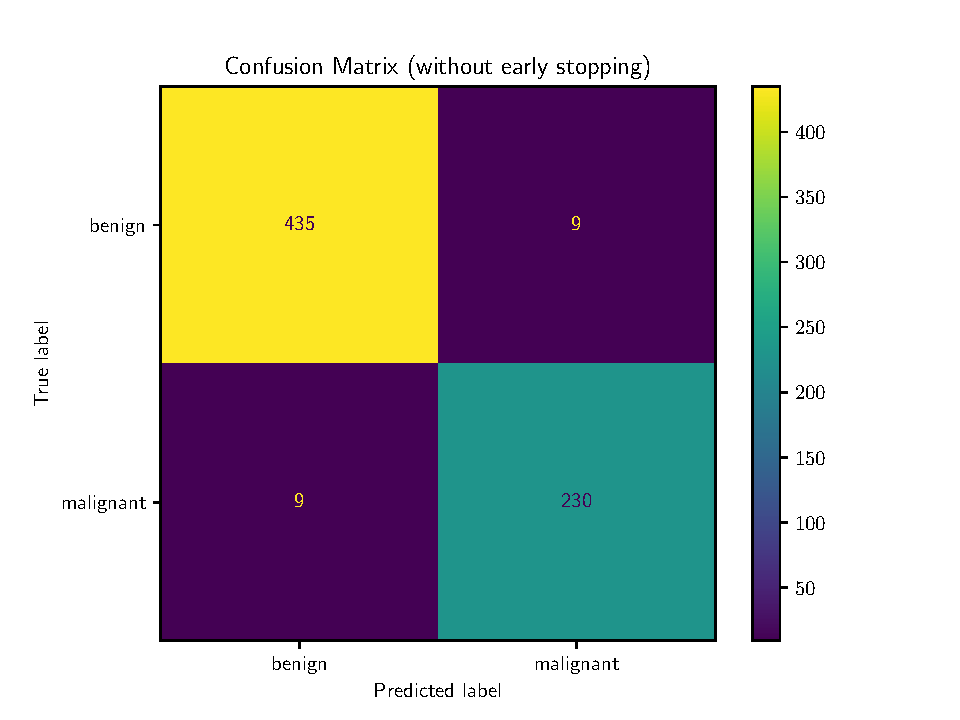
\includegraphics[width=\textwidth]{mlp_conf_matrix_False.pdf}
              %\caption{Confusion Matrix without early stopping}
            \end{minipage}
            \begin{minipage}[b]{0.49\textwidth}
              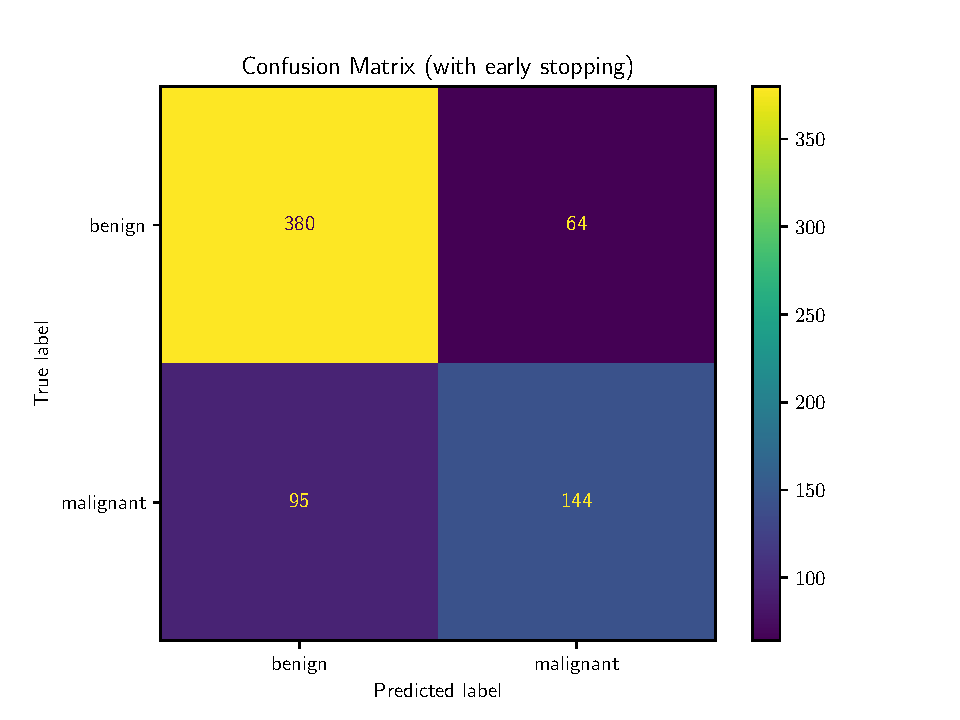
\includegraphics[width=\textwidth]{mlp_conf_matrix_True.pdf}
              %\caption{Confusion Matrix with early stopping}
            \end{minipage}
        \end{figure}
        \vspace{-1em}
        The confusion matrices above reveal a decrease in accuracy when there is early stopping, which may be due to:
        \vspace{-0.5em}
        \begin{itemize}
            \item the presence of overfitting to the validation sets across dataset folds, since early stopping aims to maximize accuracy over these subsets.
            \item the scarcity of instances that cover all possible values for each feature, which is exacerbated by creating yet another subset of the dataset in each fold. Consequently, some parameters may be left undertrained, leading to more misclassifications.
        \end{itemize}
        \item \quad
        \vspace{-0.45cm}
        \begin{figure}[H]
            \centering
              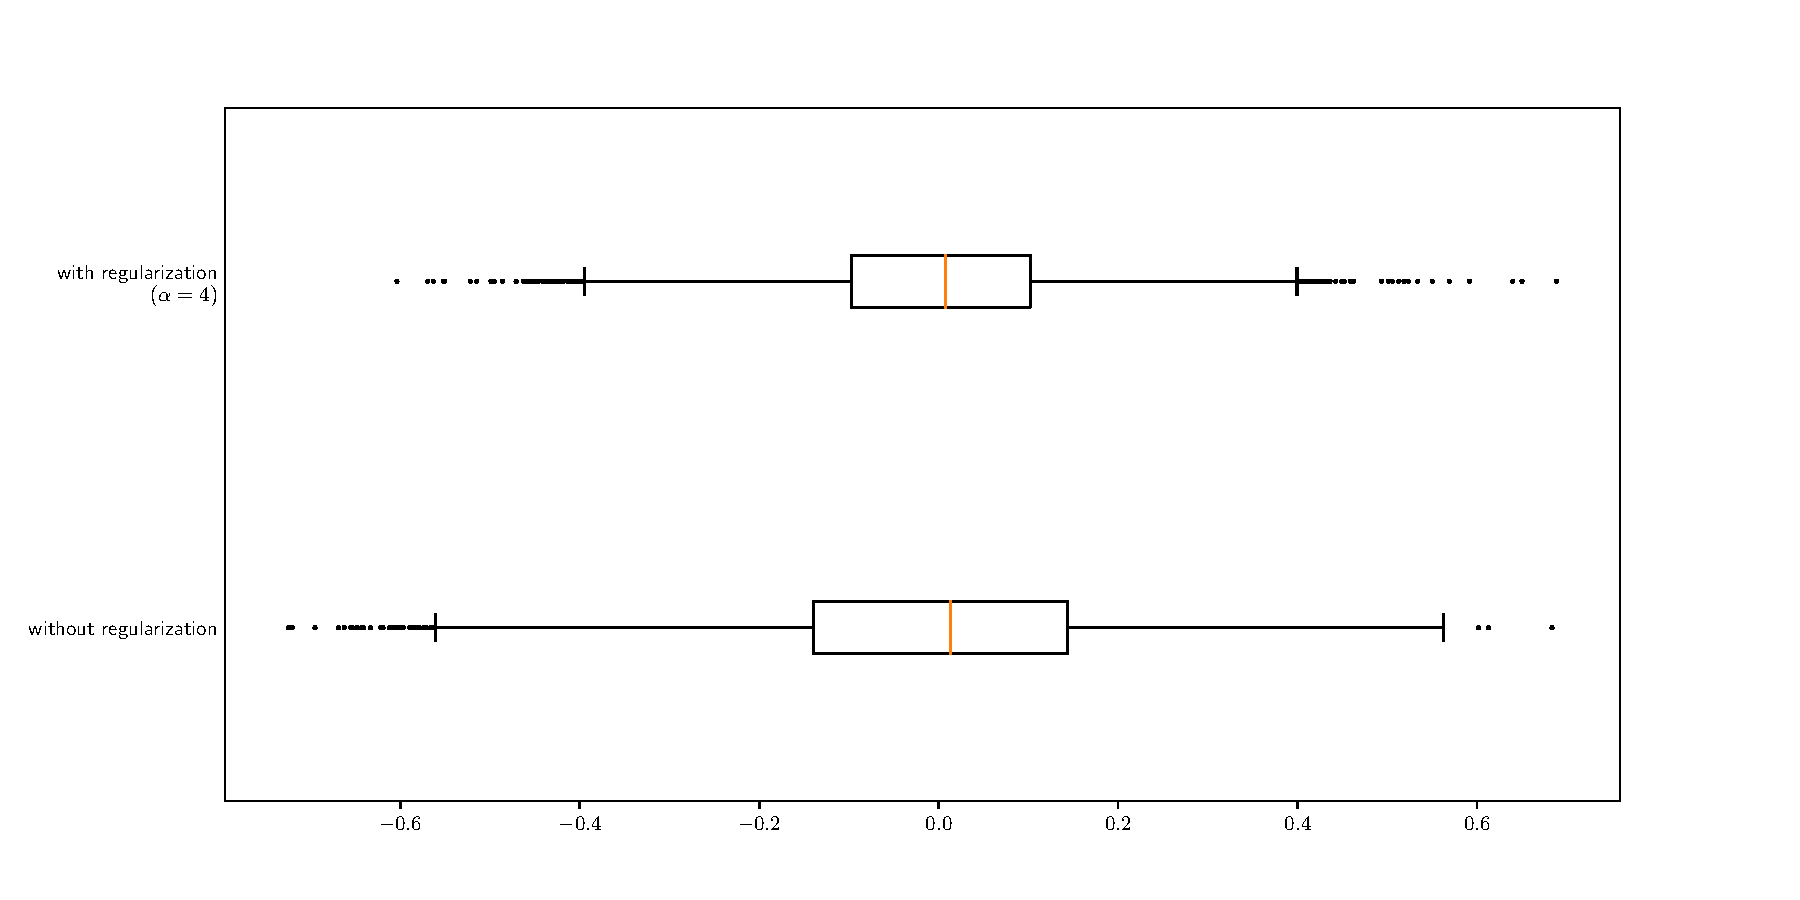
\includegraphics[width=\textwidth]{residue_boxplot.pdf}
        \end{figure}
        In order to reduce the observed error, one can:
        \begin{itemize}
            \item try different types of regularization (e.g., $l_1$ and $l_2$) so as to reduce both variability and median residue absolute value (following the plot above);
            \item tune the learning rate $\eta$ in hopes of escaping a possible local error minimum;
            \item experiment other optimization methods, such as Stochastic Gradient Descent, with or without momentum;
            \item try out different architectures, increasing both the number of layers and/or number of units per layer.
        \end{itemize}
          
    \end{questions}

    \pagebreak
    \section{Appendix}
    \inputminted{python}{src/ex02.py}
   
    
    
\end{document}